\documentclass[]{article}
\usepackage{lmodern}
\usepackage{amssymb,amsmath}
\usepackage{ifxetex,ifluatex}
\usepackage{fixltx2e} % provides \textsubscript
\ifnum 0\ifxetex 1\fi\ifluatex 1\fi=0 % if pdftex
  \usepackage[T1]{fontenc}
  \usepackage[utf8]{inputenc}
\else % if luatex or xelatex
  \ifxetex
    \usepackage{mathspec}
    \usepackage{xltxtra,xunicode}
  \else
    \usepackage{fontspec}
  \fi
  \defaultfontfeatures{Mapping=tex-text,Scale=MatchLowercase}
  \newcommand{\euro}{€}
\fi
% use upquote if available, for straight quotes in verbatim environments
\IfFileExists{upquote.sty}{\usepackage{upquote}}{}
% use microtype if available
\IfFileExists{microtype.sty}{%
\usepackage{microtype}
\UseMicrotypeSet[protrusion]{basicmath} % disable protrusion for tt fonts
}{}
\usepackage[margin=1in]{geometry}
\usepackage{graphicx}
\makeatletter
\def\maxwidth{\ifdim\Gin@nat@width>\linewidth\linewidth\else\Gin@nat@width\fi}
\def\maxheight{\ifdim\Gin@nat@height>\textheight\textheight\else\Gin@nat@height\fi}
\makeatother
% Scale images if necessary, so that they will not overflow the page
% margins by default, and it is still possible to overwrite the defaults
% using explicit options in \includegraphics[width, height, ...]{}
\setkeys{Gin}{width=\maxwidth,height=\maxheight,keepaspectratio}
\ifxetex
  \usepackage[setpagesize=false, % page size defined by xetex
              unicode=false, % unicode breaks when used with xetex
              xetex]{hyperref}
\else
  \usepackage[unicode=true]{hyperref}
\fi
\hypersetup{breaklinks=true,
            bookmarks=true,
            pdfauthor={},
            pdftitle={Modeling Activity of Neurons from NRG recording study},
            colorlinks=true,
            citecolor=blue,
            urlcolor=blue,
            linkcolor=magenta,
            pdfborder={0 0 0}}
\urlstyle{same}  % don't use monospace font for urls
\setlength{\parindent}{0pt}
\setlength{\parskip}{6pt plus 2pt minus 1pt}
\setlength{\emergencystretch}{3em}  % prevent overfull lines
\setcounter{secnumdepth}{0}

%%% Use protect on footnotes to avoid problems with footnotes in titles
\let\rmarkdownfootnote\footnote%
\def\footnote{\protect\rmarkdownfootnote}

%%% Change title format to be more compact
\usepackage{titling}
\setlength{\droptitle}{-2em}
  \title{Modeling Activity of Neurons from NRG recording study}
  \pretitle{\vspace{\droptitle}\centering\huge}
  \posttitle{\par}
  \author{Adam Pallus, Mark Walton and Ed Freedman}
  \preauthor{}\postauthor{}
  \date{}
  \predate{}\postdate{}




\begin{document}

\maketitle


\subsection{Introduction}\label{introduction}

Humans and other primates use combinations of eye and head movements to
move the line of sight. Depending on the behavioral task, different
types of movements may be employed. Gaze shifts are used to quickly
acquire a new target using a rapid head rotation combined with a
saccadic eye movement. Gaze pursuit can be used to follow a moving
target and combines head rotation with smooth pursuit eye movements.
These behaviors are often used in combination to efficiently view
objects of interest within the natural world.

Investigations of the neural correlates of these behaviors reveal that
separate neural mechanisms are employed. The superior colliculus (SC) is
a key structure in the control of gaze shifts. Experimental evidence
demonstrates that the SC contains an organized motor map that represents
a desired gaze displacement signal used to generate gaze shifts. No
analogous organized structure has been identified for pursuit movements.
Instead, pursuit seems to be controlled by a reciprocal
cerebro-ponto-cerebellar circuit. This circuit includes areas of visual
motion processing and the frontal eye fields in the cortex, pontine
nuclei that relay these signals to the cerebellum and follicular
neurons, which are likely to be responsible for generating smooth
pursuit eye movements. Although there is evidence of gaze-related
signals at each stage in this circuit, it has not been demonstrated that
these commands are used to generate head movements during pursuit.

The identification of brain regions responsible for dissociating gaze
signals into the appropriate eye and head motor commands is an ongoing
scientific pursuit. The technique of restraining the head has allowed
researchers to understand the pathways driving eye and gaze movements,
but does not distinguish between the two. When the head is free to move,
behavioral paradigms can be employed to dissociate gaze from eye-related
signals. This, combined with head-restrained studies, has allowed for
significant progress in the mapping of the oculomotor premotor circuits.
A similar method can be used to map the premotor circuits responsible
for driving head movements.

Anatomic evidence exists for the neurophysiologic basis of head control
in gaze shifts. In particular, some neurons in the reticular formation
receive inputs from the SC and project to motor neurons in the cervical
spinal cord. This places them in the ideal location to transform gaze
displacement signals from the SC into appropriate head motor commands,
though the activity of these neurons has not been described in primates
performing head-unrestrained movements.

Recordings from the medullary and pontine reticular formation in cats
have identified some neurons with activity correlated with certain
dynamics of head movement. Micro-stimulation of analogous structures in
monkeys has been shown to produce movements of the eyes, head, ears,
mouth and produce other movements, depending on the region stimulated.
Quessy and Freedman investigated a region of NRG that produces
ipsilateral horizontal head rotation when stimulated, with kinematics
similar to those observed during horizontal gaze shifts. They further
demonstrated that while stimulating these regions does not produce eye
movement directly, stimulation does alter ongoing eye movements
initiated as part of a gaze shift, implying that NRG is part of the
circuit used to produce gaze shifts.

In addition to likely gaze-shift-related inputs from the SC, NRG also
receives input from many other areas, including motor and prefrontal
cortex, the cerebellum and basal ganglia. This diversity of inputs
suggests the potential for a greater role for NRG, including the
potential for involvement in producing the head movements associated
with gaze pursuit. Cats do not employ smooth pursuit movements like
humans and monkeys do, so no physiologic evidence exists for the
activity of this region during such movements.

In this study, we return to the portion of NRG stimulated by Quessy and
Freedman to record the activity of neurons that may be responsible for
producing the head movement observed during stimulation. We use
established behavioral paradigms to dissociate gaze, eye and head
movement during gaze shifts that allow us to identify neurons whose
activity is associated with head movement apart from gaze or eye
movements. New techniques for dissociating the gaze, eye and head
movements associated with gaze pursuit are also employed, enabling us to
identify any neurons involved in producing the head movements associated
with pursuit and to determine whether these are a separate population
from those involved in producing head movements during gaze shifts. Our
behavioral paradigms also allow us to assess neurons for activity
related to eye position in the orbits. This is information required to
produce a head-specific motor command from gaze-related signals.

\subsection{Methods}\label{methods}

Two rhesus monkeys (\emph{Macaca mulatta}) served as subjects. Two
sterile surgeries were performed to prepare each animal for
neurophysiological experiments. In the first, a stainless-steel post was
affixed to the skull with bone screws, and a teflon-coated coil of wire
was implanted under the conjunctiva of one eye (Judge et al. 1980).
Following this, the monkeys were trained to perform behavioral tasks.
When they became proficient at this tasks, a second surgery was
performed to affix a recording chamber over a trephine craniotomy. The
chamber was positioned on the midline at stereotaxic zero. All surgical
and experimental procedures were approved by the University of Rochester
Animal Care and Use Committee and were in compliance with the National
Institutes of Health Guide for the Care and Use of Animals.

The data presented in this study were collected concurrently with the
behavioral data described in the previous chapter. Therefor, the
collection of behavioral data and presentation of visual targets is
identical. Briefly, monkeys were placed in a custom-designed primate
chair during experiments, that restrained the body but allowed free
movement of the head. A small, lightweight cam-lock device was attached
to the head. The position of the head was determined by the orientation
of coil of Teflon-coated wire attached to the device, using the same
method as the implanted search coil. Three red lasers attached to the
device allowed behaviral control of initial eye-in-hea position
(described in detail in previous chapter).

The monkey chair was placed in the center of a cube containing three
pairs of magnetic field coils (CNC Engineering, Seattle, WA). Signals
from the gaze and head coils were sampled at 1 kHz and filtered using a
five-pole, low-pass Bessel filter with a cutoff frequency of 3 kHz. A
second low-pass filter with a time constant of 0.3ms was applied to the
signal before digitizing. The current in the coils was linearly related
to the horizontal rotational position of the coils in the field within 2
degrees over 360 degrees.

Visual targets were presented on the inner surface of a 1.5 m hemisphere
(0.5 in acrylic; Capital Plastics, Beltsville, MD). Two additional red
lasers, attached to independent, two-axis-motorized gimbals (RGV 100
rotation stages; Newport, Irvine, CA) presented targets with \textless{}
0.01 degree accuracy. An infrared camera allowed the experimenters to
view the monkeys, which was particularly useful for assessing head-roll
during microstimulation.

\subsubsection{Neurophysiology}\label{neurophysiology}

Single neurons in NRG were isolated using a tungsten micro-electrode
(Micro Probes), amplified, filtered and saved for offline analysis. The
anterior/posterior position of the electrode in the chamber was chosen
using the characteristic firing pattern of the abducens motor nucleus as
a landmark. We close electrode tracts that traveled posterior to the
nucleus to avoid damaging motor neurons, and continued deeper. On most
tracts, the characteristic population bursting for ipsiversive gaze
shifts of PPRF was noted, as well as occasional MLBs and LLBNs. Once the
electrode was advanced beyond the level of population gaze-shift-related
activity, we also characterized the location's response to
micro-stimulation. We sought regions that produced horizontal head
rotation on stimulation, using the stimulation parameters of Quessy and
Freedman (2004) as a guide. Superficial to this region, we observed
evoked ear movements as well as head movements with vertical or roll
components. Any neurons isolated deep to the level of population gaze
activity were recorded as a candidate for inclusion in this study.

\subsubsection{Modeling}\label{modeling}

We are attempting to find a function of the recorded eye and head
movements that will predict the firing rate of the neuron during the
trial. We convert the recorded spike times into a continuous function by
convolving them with a Gaussian with a 15ms standard deviation to create
a spike density function. We scale the spike density function so that it
approximates the firing rate in spikes per second. For this analysis, we
separate leftward and rightward movements to produce 12 possible
predictor variables:
(right/left)(eye/head)(position/velocity/acceleration), represented by
the abbreviations: \emph{rhp, lhp, rep, lep, rhv, lhv, rev, lev, rha,
lha, rea} and \emph{lea}.

We use Matlab's \textbf{stepwiselm} function, beginning with a constant
model. The function evaluates the set of available terms, which includes
the predictor variables described above, as well as pairwise
interactions. If any of these terms improve the R\textsuperscript{2} of
the model by 0.05 or more, the threshold criterion we chose, it includes
the best term and then repeats the evaluation to see if any other terms
could improve the model further. If these neurons were involved in
generating the observed eye and head behavior, we assume that there
would be a time delay between neural activity and movement. We repeated
this step-wise model fitting to shifted data, in 10ms increments up to
200ms. We employed step wise fitting method to find the best fit at each
location independently. We then chose the delay that gave the best fit,
determined by the R\textsuperscript{2} weighted by the number of terms
in the model. Each additional term must improve the fit by at least
0.05. For example, if the best fit at a 50ms delay was a model with two
terms an R\textsuperscript{2} of 0.29, and the best fit at 60ms was a
model with three terms and an R\textsuperscript{2} of 0.30, we chose the
simpler model.

\subsection{Results}\label{results}

We isolated 163 neurons (94 from S and 69 from U) in NRG while monkeys
performed head-unrestrained gaze shifts and gaze pursuit tasks. The
activity of 53 of these neurons was recorded based on apparent
head-movement-related activity as perceived by the researchers during
recording, and isolation was maintained for at least 50 successful
trials. The behavior tasks that our monkeys performed provided us with a
large variety of head movements to investigate. Controlling initial eye
position provided us with examples of pursuit and gaze shifts of similar
velocities and amplitudes with varying amounts of head contribution.
This provided us with the ability to identify neurons with head-related
activity during recording. For offline analysis, we can compare the
firing rate of the neurons to the actual head and eye kinematics on a
trial-by-trial basis.

\subsubsection{Peak Firing Rate and Peak Head
Velocity}\label{peak-firing-rate-and-peak-head-velocity}

Based on the observations of the experimenters during recording, we
hypothesized that there is a correlation between the firing rate of the
neurons and the velocity of head movements. To test this hypothesis, we
first investigated the relatioship between the peak firing rate and the
peak velocity on each trial for each neuron. We identified cells that
have significant correlations between these two variables and fit linear
regression models. In figure 1, we show an example cell demonstrating
this process. Panel 1A shows the head velocity and corresponding
activity of the neuron during a fast, leftward head movement, while 1B
shows the same during a slower head movement. For each trial, we record
the peak head velocity and the peak firing rate of the neuron, which are
plotted in 1C. We fit a linear regression model for the relationship
between peak firing rate and peak velocity in each direction. For the
example neuron shown in 1C, this regression was significant
(p\textless{}0.001) for leftward movements only. Table 1 summarizes the
results of this analysis for each neuron in our population.

We find that 20 cells show a significant regression (p\textless{}0.001)
with rightward movements, 28 for leftward and 14 for both. That is a
total of 34 neurons with a significant correlation with head movements
of at least one direction. If we impose the additional requirement that
firing rate must increase with faster head movements (slope of
regression is positive for rightward and negative for leftward head
movements, we find 19 for rightward, 23 for leftward and 9 for both; a
total of 33 neurons (67\%). In figure 2, we plot regression lines for
these cells on same axes, as three groups, corresponding to whether they
are significant for leftward, rightward or both directions.

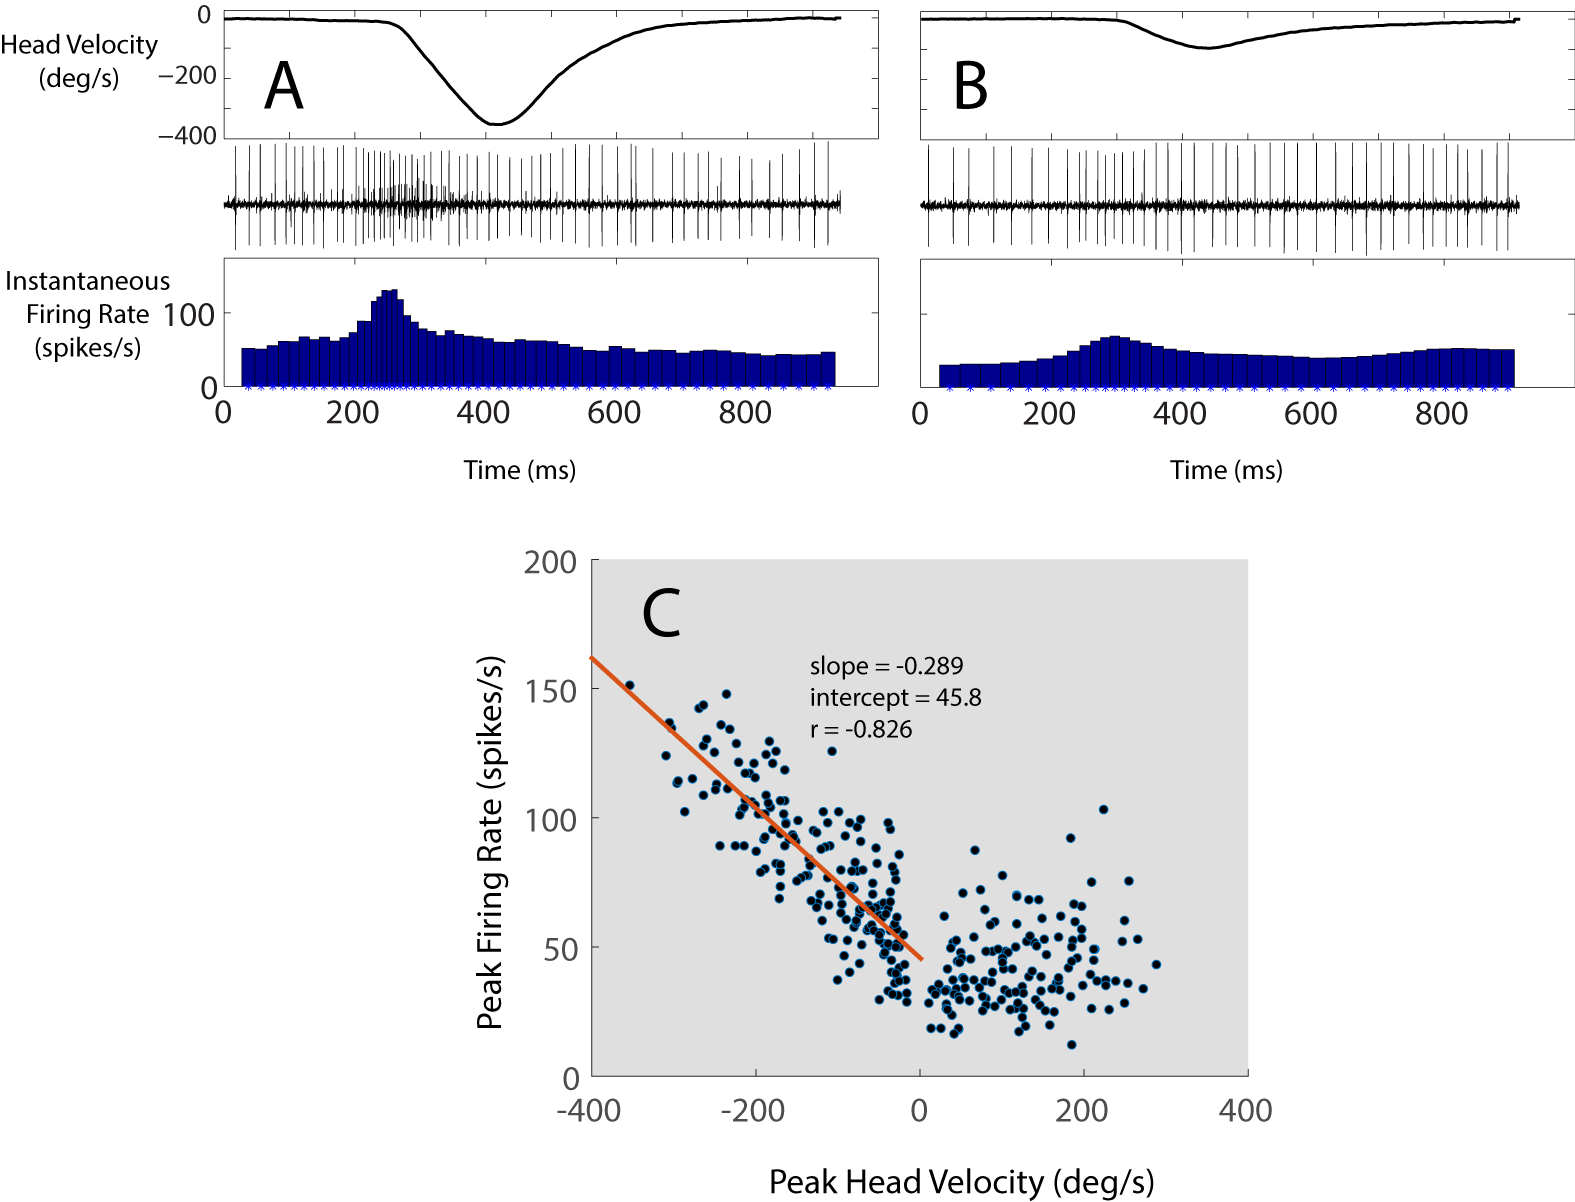
\includegraphics{Example1sc21dec11.png}

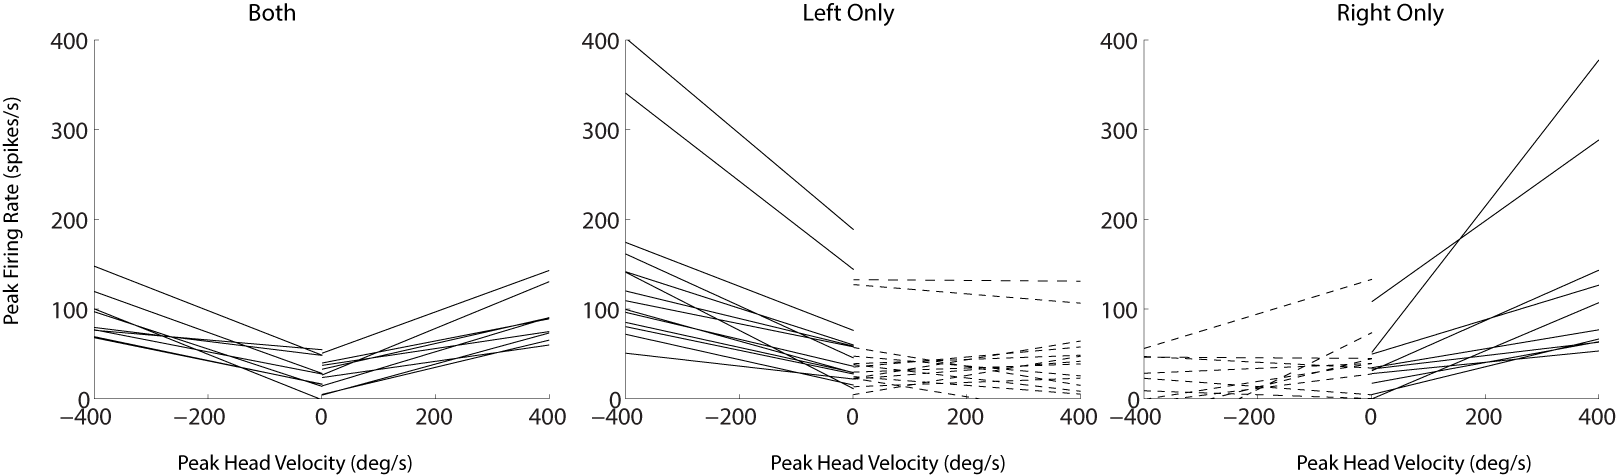
\includegraphics{peakregressions.png}

\begin{table}[ht]
\centering
\begin{tabular}{rlrrrrrrrrrr}
  \hline
 & Neuron & n.r & slope.r & intercept.r & r.r & p.r & n.l & slope.l & intercept.l & r.l & p.l \\ 
  \hline
1 & SB10Jan12 & 110 & 0.13 & 38.80 & 0.31 & 0.00 & 143 & -0.10 & 43.78 & -0.32 & 0.00 \\ 
  2 & SC12Dec11 & 133 & 0.08 & 35.22 & 0.34 & 0.00 & 151 & -0.32 & 36.80 & -0.81 & 0.00 \\ 
  3 & SD04Jan12 & 287 & 0.10 & 20.67 & 0.27 & 0.00 & 283 & -0.12 & 15.75 & -0.49 & 0.00 \\ 
  4 & SD21Sep11 & 114 & 0.19 & 23.82 & 0.50 & 0.00 & 180 & -0.11 & 41.77 & -0.51 & 0.00 \\ 
  5 & UB22may12 &  66 & 0.16 & 17.01 & 0.81 & 0.00 &  60 & -0.19 & 16.10 & -0.83 & 0.00 \\ 
  6 & UB23mar12 &  66 & 0.17 & -1.19 & 0.66 & 0.00 &  55 & -0.16 & 20.32 & -0.73 & 0.00 \\ 
  7 & UB24oct11 & 121 & 0.11 & 38.84 & 0.39 & 0.00 &  97 & -0.10 & 32.30 & -0.41 & 0.00 \\ 
  8 & UC17feb12 & 364 & 0.18 & -4.48 & 0.65 & 0.00 & 141 & -0.26 & -7.50 & -0.85 & 0.00 \\ 
  9 & SB10Oct11 & 223 & 0.47 & 102.25 & 0.62 & 0.00 & 170 & 0.14 & 37.19 & 0.46 & 0.00 \\ 
  10 & SB21Oct11 &  94 & 1.09 & 4.07 & 0.84 & 0.00 &  63 & 0.35 & 70.90 & 0.53 & 0.00 \\ 
  11 & SC14Oct11 & 168 & 0.06 & 28.64 & 0.29 & 0.00 & 121 & 0.09 & 27.00 & 0.37 & 0.00 \\ 
  12 & SC18Oct11 & 181 & 0.40 & 15.93 & 0.52 & 0.00 & 133 & 0.12 & 33.42 & 0.48 & 0.00 \\ 
  13 & UD16sep11 & 133 & -0.07 & 25.27 & -0.32 & 0.00 & 194 & -0.17 & 50.48 & -0.40 & 0.00 \\ 
  14 & SB16Sep11 &  45 & 0.12 & -0.72 & 0.33 & 0.03 &  64 & -0.23 & 16.32 & -0.74 & 0.00 \\ 
  15 & SB19Jan12 & 116 & 0.16 & 2.51 & 0.62 & 0.00 &  87 & -0.05 & 4.36 & -0.19 & 0.07 \\ 
  16 & SB28Sep11 &  75 & 0.42 & 25.60 & 0.53 & 0.00 &  39 & 0.08 & 54.22 & 0.08 & 0.63 \\ 
  17 & SC07Oct11 & 103 & 0.15 & 35.73 & 0.21 & 0.03 &  78 & -0.17 & 32.85 & -0.57 & 0.00 \\ 
  18 & SC21Dec11 & 140 & 0.09 & 34.86 & 0.24 & 0.00 & 183 & -0.30 & 41.31 & -0.68 & 0.00 \\ 
  19 & SC23Sep11 &  67 & -0.05 & 41.82 & -0.18 & 0.13 & 163 & -0.20 & 78.57 & -0.39 & 0.00 \\ 
  20 & SD03Nov11 & 111 & 0.40 & -18.97 & 0.41 & 0.00 & 132 & 0.39 & 175.69 & 0.24 & 0.01 \\ 
  21 & SD09Jan12 & 104 & -0.14 & 55.26 & -0.28 & 0.00 & 156 & -0.51 & 131.46 & -0.31 & 0.00 \\ 
  22 & SD13Jan12 &  90 & 0.01 & 145.90 & 0.00 & 0.97 & 158 & -0.62 & 201.51 & -0.35 & 0.00 \\ 
  23 & UB05jan12 & 201 & 0.28 & 28.74 & 0.56 & 0.00 & 244 & -0.03 & 64.31 & -0.07 & 0.27 \\ 
  24 & UB07oct11 &  94 & 0.41 & 44.05 & 0.48 & 0.00 &  95 & -0.29 & 45.23 & -0.27 & 0.01 \\ 
  25 & UB11jan12 &  56 & 0.16 & 71.32 & 0.20 & 0.14 &  95 & -0.41 & 33.07 & -0.39 & 0.00 \\ 
  26 & UB16feb12 & 258 & -0.02 & 11.41 & -0.15 & 0.02 &  97 & -0.18 & 50.08 & -0.45 & 0.00 \\ 
  27 & UB26mar12 & 199 & 0.11 & 28.30 & 0.12 & 0.08 & 157 & -0.20 & 20.82 & -0.54 & 0.00 \\ 
  28 & UE31oct11 &  39 & 0.06 & 17.70 & 0.55 & 0.00 &  27 & -0.24 & 10.85 & -0.47 & 0.01 \\ 
  29 & SB05Oct11 & 138 & 0.03 & 50.95 & 0.05 & 0.56 &  92 & -0.06 & 48.56 & -0.15 & 0.14 \\ 
  30 & SB07Oct11 &  38 & 0.09 & 36.03 & 0.22 & 0.18 &  33 & 0.01 & 28.60 & 0.04 & 0.83 \\ 
  31 & SB15Sep11 &  57 & 0.14 & 19.44 & 0.31 & 0.02 &  45 & -0.01 & -0.26 & -0.19 & 0.21 \\ 
  32 & SB18Oct11 &  48 & 0.04 & 62.02 & 0.07 & 0.65 &  44 & -0.02 & 24.24 & -0.08 & 0.60 \\ 
  33 & SB30Sep11 & 114 & 0.26 & 5.34 & 0.24 & 0.01 &  82 & -0.05 & -0.50 & -0.22 & 0.05 \\ 
  34 & SC19Jan12 &  76 & -0.09 & 20.39 & -0.32 & 0.01 & 151 & -0.12 & 20.49 & -0.13 & 0.10 \\ 
  35 & SC19Oct11 &  65 & 0.05 & 30.30 & 0.27 & 0.03 &  44 & -0.03 & 19.61 & -0.07 & 0.65 \\ 
  36 & SC28Nov11 & 199 & 0.10 & 22.35 & 0.21 & 0.00 & 171 & 0.01 & 50.18 & 0.01 & 0.85 \\ 
  37 & SD06Dec11 & 109 & 0.03 & 64.29 & 0.02 & 0.81 &  74 & -0.46 & 45.14 & -0.23 & 0.05 \\ 
  38 & SD28Sep11 &  89 & 0.01 & 29.83 & 0.07 & 0.51 &  64 & -0.04 & 17.27 & -0.25 & 0.05 \\ 
  39 & SD30Sep11 & 103 & 0.08 & 301.71 & 0.05 & 0.62 &  67 & -0.37 & 110.74 & -0.22 & 0.08 \\ 
  40 & SE17Oct11 &  59 & 0.14 & 48.52 & 0.34 & 0.01 &  45 & 0.05 & 10.66 & 0.31 & 0.04 \\ 
  41 & UB04nov11 &  68 & 0.08 & 39.97 & 0.22 & 0.07 &  54 & -0.00 & 35.97 & -0.01 & 0.96 \\ 
  42 & UC03jan12 &  24 & 0.10 & 27.95 & 0.28 & 0.19 &  74 & -0.05 & 65.04 & -0.05 & 0.67 \\ 
   \hline
\end{tabular}
\caption{Results of linear regression modeling between peak head velocity and peak firing rate of each neuron. } 
\end{table}

\paragraph{Pursuit vs Gaze shift
activity}\label{pursuit-vs-gaze-shift-activity}

One question we sought to answer when designing these experiments
regarded whether the neurons in NRG were participating in head movements
made during both gaze shifts and pursuit. An alternative is that NRG
activity is dependent on SC activity and therefore only active during
gaze shifts. General observation did not reveal any neurons with
activity limited to only head movements associated with one behavioral
task. Despite this, some neurons seemed to fire more rapidly during
pursuit movements, even though the head movements were faster.

\subsubsection{Eye Position}\label{eye-position}

Observation of the fixation prior to movement initiation indicates
position-related firing in several neurons. We use anova to identify
cells with significantly different firing rates for the three different
combination of eye and head positions in use during fixation. To
determine whether this firing is due to eye or head position, we must
compare to other parts of the trial, such as at the end of a gaze shift
when the eyes are centered and the head is eccentric.

\subsubsection{Modeling}\label{modeling-1}

The above analysis was restricted to the peak firing rate of the neuron
on each trial. Further, it assumes that head velocity is an important
factor for each neuron. In this section, we use the unbiased modeling
approach described in detail in \emph{Methods}. For 51 of the 53 neurons
included in this study, we were able to model firing rate as a function
of eye or head position, velocity or acceleration. For the neurons we
were unable to fit, this means that no individual term improved the
variance accounted for (R\textsuperscript{2}) of the constant model by
0.05 or better, suggesting that these neurons do not have activity
related to eye or head movements. The table below shows the shift (the
delay between cell activity and the eye and head paramters being
modeled), the R\textsuperscript{2} indicating goodness of fit, and the
formula. Although we allowed for interaction terms in our step-wise
fitting procedure, we do not observe interactions.

\begin{table}[ht]
\centering
\begin{tabular}{rlrrl}
  \hline
 & Neuron & shift & rsquared & f \\ 
  \hline
1 & SB21Oct11 & 120 & 0.77 & fr \~{} 1 + rhv + rep \\ 
  2 & UB21dec11 &  60 & 0.70 & fr \~{} 1 + lep \\ 
  3 & UB22may12 &  70 & 0.64 & fr \~{} 1 + rhv + lhv \\ 
  4 & SE17Oct11 & 150 & 0.58 & fr \~{} 1 + rhv \\ 
  5 & SB10Oct11 & 170 & 0.58 & fr \~{} 1 + rhp + rhv \\ 
  6 & UC22may12 &  80 & 0.57 & fr \~{} 1 + rhv + lhv \\ 
  7 & SC23Sep11 & 130 & 0.47 & fr \~{} 1 + lhv \\ 
  8 & UBA4jun12 &  90 & 0.46 & fr \~{} 1 + rhv + lhv \\ 
  9 & SD09Jan12 & 130 & 0.41 & fr \~{} 1 + lhv \\ 
  10 & UB23mar12 &  80 & 0.40 & fr \~{} 1 + lhv + rep \\ 
  11 & SC12Dec11 &  70 & 0.40 & fr \~{} 1 + lhv \\ 
  12 & UB16feb12 &  90 & 0.40 & fr \~{} 1 + lhv \\ 
  13 & UB05jan12 &  60 & 0.39 & fr \~{} 1 + lhp + lhv + rha \\ 
  14 & SB15Sep11 & 110 & 0.37 & fr \~{} 1 + rhv \\ 
  15 & UB28sep11 &  20 & 0.35 & fr \~{} 1 + rhp + rhv + rep \\ 
  16 & SD03Nov11 & 160 & 0.34 & fr \~{} 1 + lhv \\ 
  17 & SC18Oct11 &  40 & 0.33 & fr \~{} 1 + rhv + lep \\ 
  18 & SB16Sep11 &  70 & 0.32 & fr \~{} 1 + lhv \\ 
  19 & UD16sep11 & 130 & 0.32 & fr \~{} 1 + lhv \\ 
  20 & UB04nov11 &  70 & 0.31 & fr \~{} 1 + rhv + lhv \\ 
   \hline
\end{tabular}
\caption{This table shows the results of a step-wise fitting procedure that with a threshold for inclusion of an increase of 0.5 in the R2} 
\end{table}

The histogram below shows the distribution the shifts obtained with this
method. The shift represents the separation between the firing rate of
the neuron and the eye and head behavior. We hypothesize that this is
approximately the latency between the activity and the movements being
generated by the activity, but only for cells that are actually involved
in generating these movements. The average shift was 95.47ms, with a
standard deviation of 47.25.

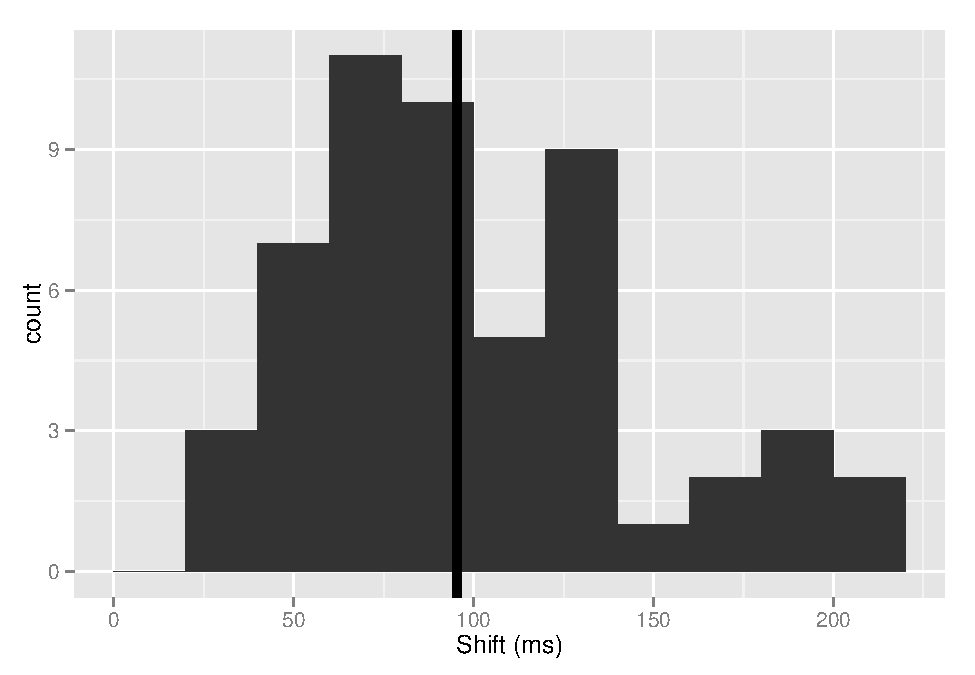
\includegraphics{NRGRecord_files/figure-latex/shift_histogram-1.pdf}

The next histogram (below), summarizes how well the models fit the
activity of the neurons. The average R\textsuperscript{2} was 0.29, with
a standard deviation of 0.17.

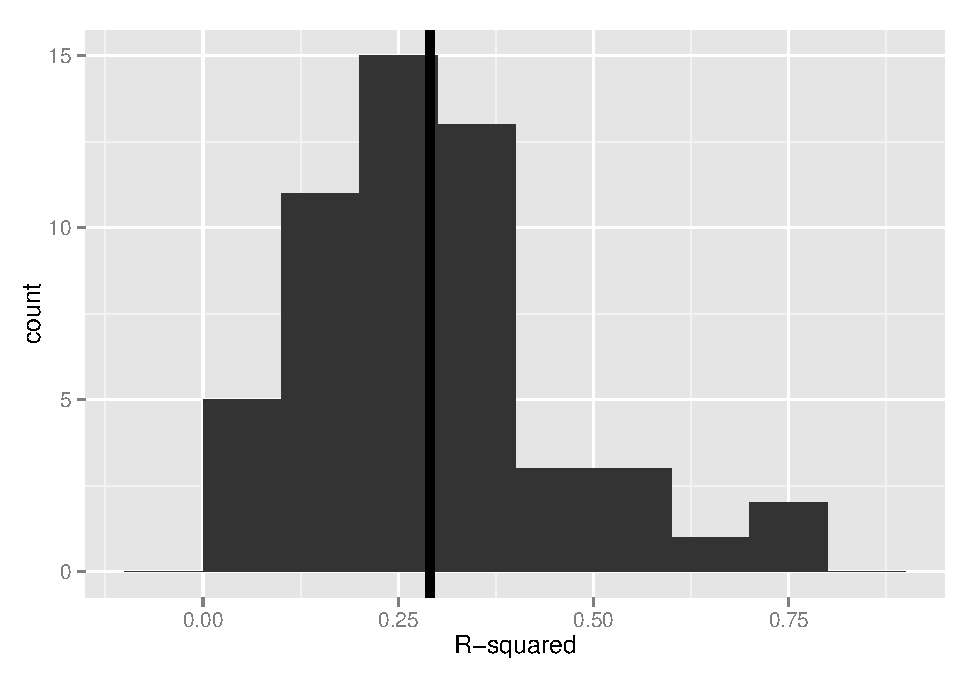
\includegraphics{NRGRecord_files/figure-latex/rsquared_histogram-1.pdf}

From the above table, it is clear that several different models were
found to best describe the neurons in our population. The histogram
below indicates how often each particular model appears in our data set.

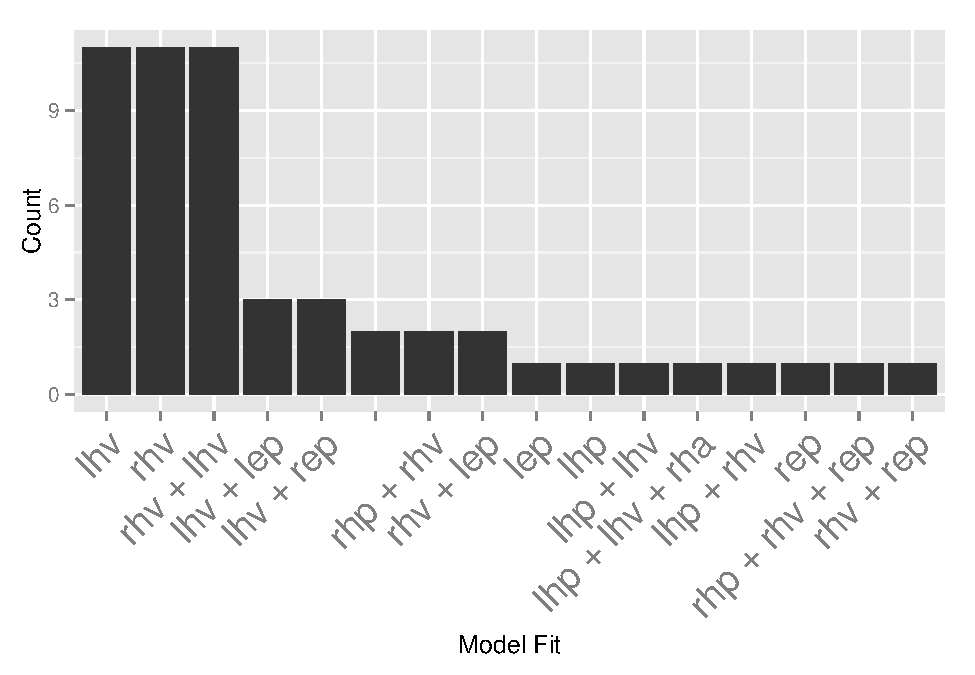
\includegraphics{NRGRecord_files/figure-latex/modelcount-1.pdf}

From this analysis, it appears that many different models are used, but
there is a lot of similarity.

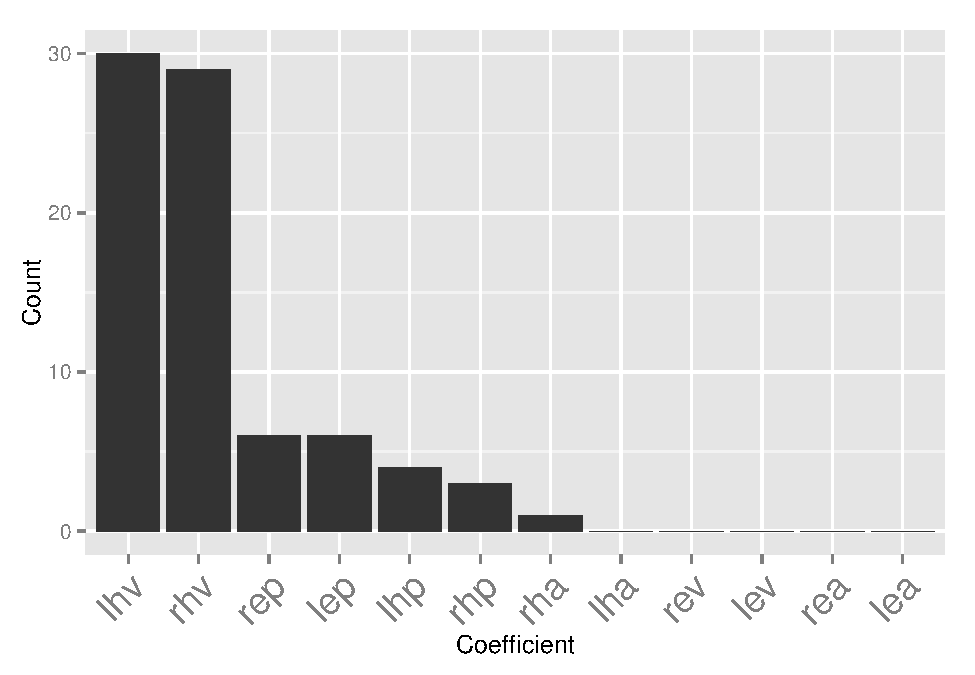
\includegraphics{NRGRecord_files/figure-latex/coefCounts-1.pdf}

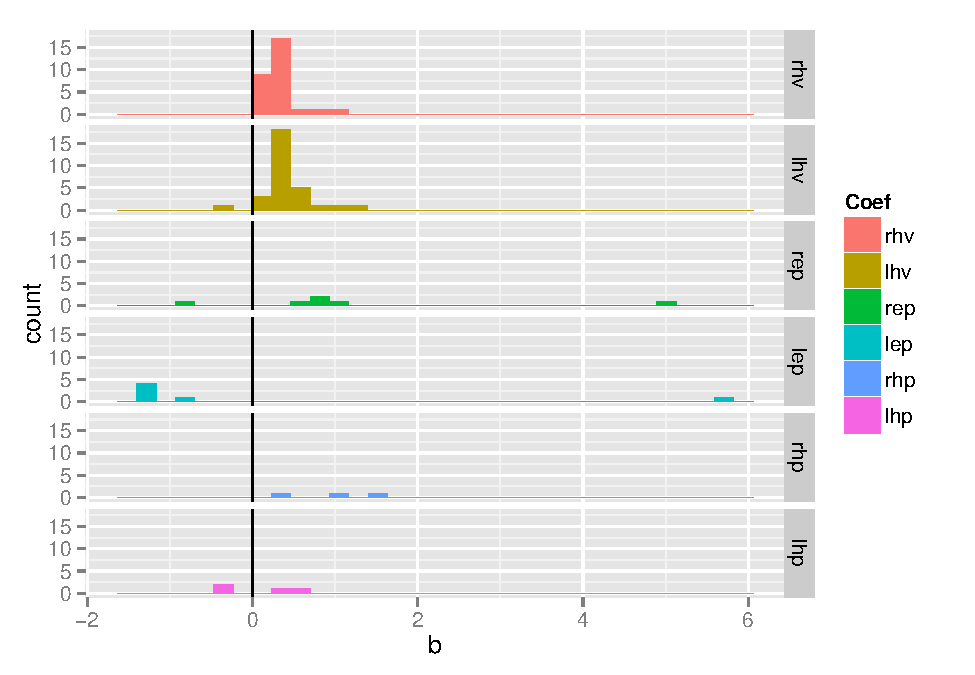
\includegraphics{NRGRecord_files/figure-latex/hvCoefs-1.pdf}

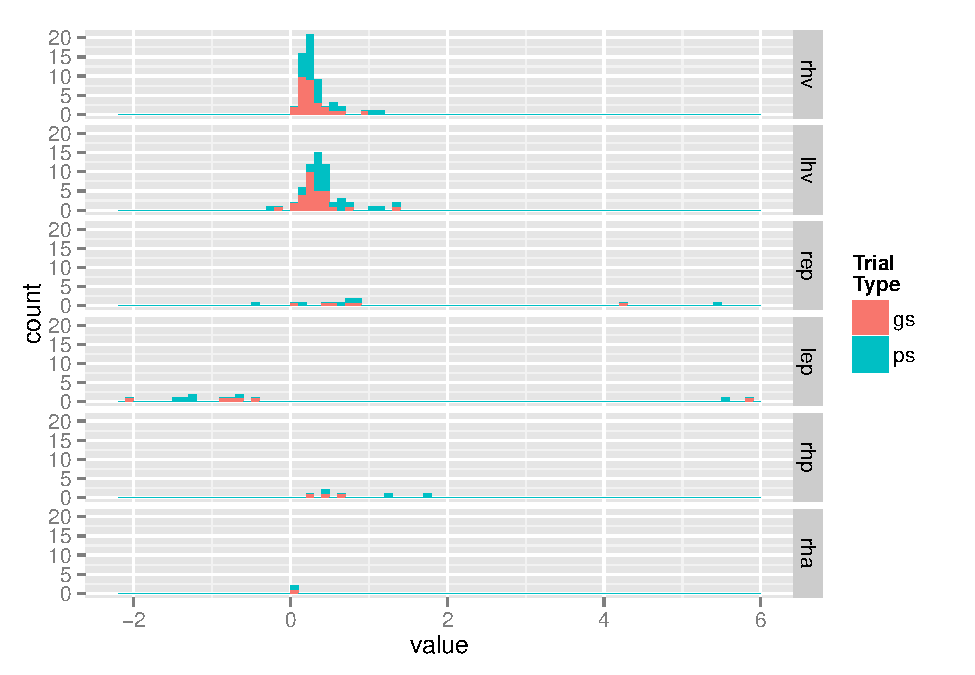
\includegraphics{NRGRecord_files/figure-latex/gspdiff-1.pdf}

What I did in the above figure was fit a linear model to gaze shift
trials and pursuit trials individually, with the same formula and shift
as determined by stepwise fit procedure. This shows that the
coefficients are similar for trials of the different types. None of the
differences are significant. Might want to show box plot.

Next plot I would consider doing is running the whole stepwise procedure
over and allowing the shift to be anything, then comparing how the fits
differ.

\subsection{Discussion}\label{discussion}

In this experiment, we examined the activity of neurons in a head
movement-related area of the brainstem: the nucleus reticularis
gigantocellularis (NRG). We recorded the firing patterns of individual
neurons in this region while subjects performed head-unrestrained gaze
movements, which included gaze shifts and gaze pursuit. We evoked these
movements using two behavioral tasks, a standard delayed gaze shift task
(See: Freedman and sparks 1997, walton and freedman 2014), and a visual
tracking task that subjects accomplished using a combination of smooth
gaze pursuit and catch-up saccades (gaze shifts).

Including pursuit behavior in this study allows us to evaluate whether
particular inputs to the region are driving the head movements we
observe. The activity of the superior colliculus (SC) is well documented
during head unrestrained gaze shifts. During such movements, the deeper
layers of the SC has been shown to encode a gaze displacement signal,
which correlates with the amplitude of the gaze shift without regard for
the combination of eye and head movements that are used to execute it.
This implies that regions downstream from the SC transform this gaze
amplitude information into appropriate eye and head motor commands. The
NRG has been proposed as a region that could perform this transformation
for the head movement portion of gaze shifts, based on the monosynaptic
connections between the SC and NRG and the NRG to neck motor neurons in
the brain stem, in addition to the observed head rotation evoked by
stimulation of NRG. Such a hypothesis predicts that the activity of NRG
is related to the head movement during gaze shifts. Our results show
that many neurons in NRG do have activity that is well correlated with
head velocity during gaze shifts.

During the visual tracking task, neural activity is also correlated with
head velocity. This activity is unlikely to be a result of input from
the SC, which is not involved in generating the smooth gaze movements
seen during pursuit. SC activity is likely to be responsible for
producing catch-up gaze shifts, but these are small amplitude movements
that would not be associated with the large head movements observed
during pursuit. This suggests that input from a region other than the SC
is responsible for the head velocity-related activity observed in the
NRG. This input could come from gaze pursuit pathways, such as the
FEF/MT-\textgreater{} NRTP/DLPN-\textgreater{} Cerebellum-\textgreater{}
brainstem pathway that has been shown to be involved in both smooth
pursuit eye movements and head-unrestrained gaze pursuit. It has been
proposed that a head-velocity command could be generated from this
pathway (Ackerly and Barnes 2011), so the NRG could represent a
convergence of the gaze shift and pursuit pathways.

Several lines of evidence demonstrate that gaze amplitude alone is
insufficient to determine the head movement associated with a gaze
shift. Information about the initial positions of the eyes in the orbits
is also required to generate the appropriate head amplitude. We find
evidence of eye position-related activity in a portion of the neurons we
recorded. We hypothesize that this represents monitoring of the position
of the eyes, rather than evidence that the NRG is responsible for
generating eye movements. With this information available, the NRG

We have recently shown (Pallus and Freedman 2015) that head movements
during pursuit are influenced by both the velocity of the target and the
position of the target relative to the head, which can be determined
using the positions of the eyes in the orbits. This conclusion is
inconsistent with models of gaze pursuit that derive a head movement
command from the gaze pursuit pathway, since desired gaze pursuit
velocity is independent of the position of the target. However, the eye
position-related signals we find in this region of the NRG could allow
it to generate the appropriate head commands by combining these
position-related signals with the velocity-related signals from the
pursuit pathway.

Although we found that the activity of cells in our data set were
correlated with head velocity regardless of the behavior task, we also
observed differences in the relationship between firing rate and head
velocity. In some individual cells, the difference was obvious, but
statistical tests revealed significant differences in many of our cells.
This is difficult to explain given the assumption that activity in NRG
is responsible for driving head movements. One possibility is that the
cells are sensitive to an aspect of head movement that is different
between movement types. In our modeling analysis, we considered head
position, velocity and acceleration, but were unable to account for the
observed differences. We also allowed for the possibility that eye
movements could be responsible for the differences, but found that
neither eye position, velocity nor acceleration could account for the
differences. Instead, we find that the sensitivity to head velocity of a
subset of our neurons is higher on trials requiring visual tracking
compared to the delayed gaze shift task.

\end{document}
